%*****************************************
% Lab 08: Reaction Timer
%*****************************************
\chapter{Reaction Timer}

\section{Purpose}

This lab continues the exploration of timing circuits and is intended to provide additional practice with sequential circuit design. The project is to build a circuit that times a user's reaction speed. When complete, the \lstinline[columns=fixed]|main| circuit should look something like Figure \ref{fig:08-01}.

\begin{figure}[H]
	\centering
	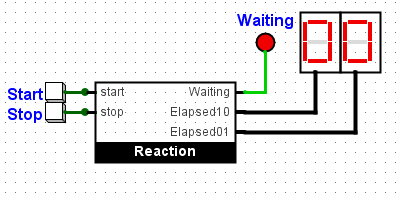
\includegraphics[width=\maxwidth{.95\linewidth}]{gfx/08-01}
	\caption{Reaction Timer}
	\label{fig:08-01}
\end{figure}

In operation:

\begin{enumerate}
	\item The user clicks \textit{start}. 
	\item An unseen timer begins and counts down a random length of time while the ``Waiting'' LED is lit. The countdown should be less than 10 seconds so use a 4-bit counter for this part of the circuit.
	\item When the unseen timer reaches zero the ``Waiting'' LED turns off and the numbers on the two hex displays begin to increase.
	\item The user clicks the \textit{Stop} button to stop the timer.
	\item The reaction time is displayed on the two hex displays.
\end{enumerate}

\section{Procedure}

The design of this circuit is left to the student, but the timer built in Lab 7 would be a good starter for this lab. As a tip, \LE includes a Random Generator (\textit{Memory} library) that can be used to create a random countdown for the ``Waiting'' subcircuit. Finally, the \textsc{Simulate -> Tick Frequency} can be set to a low number (maybe 4 Hz) to build and troubleshoot the circuit for convenience but it should then be set somewhat faster to actually measure a user's reaction time.

\section{Deliverable}

To receive a grade for this lab, complete the circuit. Be sure the standard identifying information is at the top left of the \lstinline{main} circuit, similar to: 

\bigskip
% The minipage environment keeps the three lines together - no page break.
\begin{minipage}{\linewidth}
	\begin{verbatim}
	George Self
	Lab 08: React
	March 11, 2018
	\end{verbatim}
\end{minipage}
\bigskip

Save the file with this name: \emph{\texttt{Lab08\_React}} and submit that file for grading.

